\documentclass[11pt]{report}

\usepackage[style=ieee]{biblatex}
\usepackage{graphicx}
\usepackage{pgfplots}
\pgfplotsset{compat=1.15}
\usepackage{caption}
\usepackage{subcaption}
\usepackage[T1]{fontenc}
\usepackage{graphicx}
\usepackage{tabu}
\usepackage{longtable}
\usepackage{wrapfig}
\usepackage{pdfpages}
\usepackage[utf8]{inputenc}
\usepackage{gensymb}
\usepackage[a4paper, left=30mm, right=30mm, top=25mm, bottom=25mm]{geometry}
\usepackage{titling}
\usepackage[symbols,nonumberlist,nogroupskip,shortcuts=other, xindy]{glossaries-extra}
\usepackage{fancyhdr}
\pagestyle{fancy}

\title{Synthetic aperture imaging radar signal simulation of urban environments}
\author{Thomas Stenson Moffat}

\fancyhead{}
\fancyhead[R]{\thetitle}
\fancyfoot{}
\fancyfoot[R]{\thepage}
\fancyfoot[L] {Part \thechapter}
\fancyfoot[C]{\theauthor}


\renewcommand{\chaptername}{Part}

\addbibresource{../FYP.bib}

\tabulinesep=1mm

\makeglossaries

%Add in new symbols here: (command is \newsym[description={position}]{x}{\ensuremath{x}} and reference with \gls{label}
\newsym[description={position}]{x_pos}{\ensuremath{x}}
\newsym[description={Noise equivalent}]{sigma0}{\ensuremath{\sigma^0}}
\newsym[description={Light speed in a vacuum}]{c}{\ensuremath{c}}
\newsym[description={Bandwidth of the signal}]{B}{\ensuremath{B}}
\newsym[description={Wavelength of the signal}]{lambda}{\ensuremath{\lambda}}
\newsym[description={Radial resolution}]{DeltaR}{\ensuremath{\Delta R}}
\newsym[description={Ground resolution}]{DeltaRg}{\ensuremath{\Delta R_g}}
\newsym[description={Angle from horizontal to beam centre}]{alpha}{\ensuremath{\alpha}}
\newsym[description={Beam elevation angle}]{thetael}{\ensuremath{\theta _{el}}}
\newsym[description={Swath length}]{Ls}{\ensuremath{Ls}}
\newsym[description={Azimuthal angle}]{thetaaz}{\ensuremath{\theta_{az}}}
\newsym[description={Aperture size in desired dimension}]{D}{\ensuremath{D}}
\newsym[description={Angular wave number (i.e. $\frac{2\pi}{r}$)}]{k0}{\ensuremath{k_0}}
\newsym[description={2-way phase history}]{phix}{\ensuremath{\phi(x)}}
\newsym[description={Center distance of the beam}]{r0}{\ensuremath{r_0}}
\newsym[description={Total displacement of the platform}]{x}{\ensuremath{x}}
\newsym[description={Outer radial distance of the beam}]{r}{\ensuremath{r}}
\newsym[description={Difference between r and $r_0$}]{deltar}{\ensuremath{\Delta r}}
\newsym[description={Synthesised beam width}]{thetasa}{\ensuremath{\theta _{sa}}}
\newsym[description={Cross-range resolution}]{deltax}{\ensuremath{\Delta x}}
\newsym[description={Transmitter power}]{Pt}{\ensuremath{P_t}}
\newsym[description={Range}]{R}{\ensuremath{R}}
\newsym[description={Transmitter gain}]{Gt}{\ensuremath{G_t}}
\newsym[description={Radar cross-section}]{sigmab}{\ensuremath{\sigma _b}}
\newsym[description={Effective antenna aperture area}]{Ae}{\ensuremath{A_e}}
\newsym[description={Received gain}]{Gr}{\ensuremath{G_r}}
\newsym[description={Total gain}]{G}{\ensuremath{G}}
\newsym[description={Maximum range}]{Rmax}{\ensuremath{R_\text{max}}}
\newsym[description={Minimum detectable signal}]{Pmin}{\ensuremath{P_\text{min}}}
\newsym[description={Boltzmann's constant}]{k}{\ensuremath{k}}
\newsym[description={System noise temperature}]{Tsys}{\ensuremath{T_\text{sys}}}
\newsym[description={Noise power}]{Pn}{\ensuremath{P_n}}
\newsym[description={Pulse width}]{tau}{\ensuremath{\tau}}
\newsym[description={A number}]{n}{\ensuremath{n}}
\newsym[description={Average power across all pulses}]{Pav}{\ensuremath{P_{av}}}
\newsym[description={Time spent observing the target}]{tobs}{\ensuremath{T_{obs}}}
\newsym[description={Platform velocity}]{vp}{\ensuremath{v_p}}

\begin{document}



\begin{titlepage}
	\begin{center}
	\vspace*{2cm}
	\Huge
	\textbf{\thetitle}\\
	\vspace{2cm}
	\LARGE
	\textsc{\textbf{\theauthor}}\\
	11501
	
	\vspace{2cm}
	
	
\includegraphics{../figures/uob_logo_high_res}
	
	\vspace{3cm}
	
	MEng final individual project report\\
	\vfill
	Academic Year 2020-2021\\
	Dr Robert Watson\\
	
	Wordcount: 
	\end{center}
	
\end{titlepage}

\section*{Abstract}
\newpage
\tableofcontents
\listoffigures
\printglossary[type=symbols,style=long,title={List of Symbols}]
\chapter{Introduction}
\chapter{Engineering Analysis}
\section{Introduction to SAR}

Synthetic aperture radar (SAR) is a method of radar imaging that allows for a greater dimension of radar aperture than is possible in a single element or an array of elements. This is generally achieved by mounting a radar transceiver to a moving platform and moving it past the target to be imaged however the transceiver can be stationary and the target moved past it. The image uses the relative movement between the platform and the target to build up an image based on the responses received and then time multiplexing all the responses. This movement, and hence the larger aperture created, allows for a finer spatial resolution than can be achieved by more conventional beam scanning radar. These images can be useful for a variety of applications such as remote mapping of the surface of the Earth for glaciology and geology among others. Interferometric SAR can also be used to create elevation maps by taking two measurements from different positions and comparing the differences.
Simulating a SAR image is desirable as flight time can be expensive and time consuming to get quality images so defining the flight paths and angles before any imaging is carried out saves both time and money. \par
There are two main methods of imaging using SAR. These are stripmap and spotlight imaging. Stripmap imaging SAR keeps the radar beam fixed at 90\degree to the direction of travel of the platform to which it is mounted, giving an even resolution image over the entire imaging area. Spotlight SAR uses beam steering in order to focus on one specific area to increase image resolution in that area, at the expense of image resolution in other areas. This extra time spent focusing on the single area increases the synthetic aperture length for that section only which increases the resolution.

\begin{figure}
	\centering
	\begin{subfigure}{.5\textwidth}
	\centering
	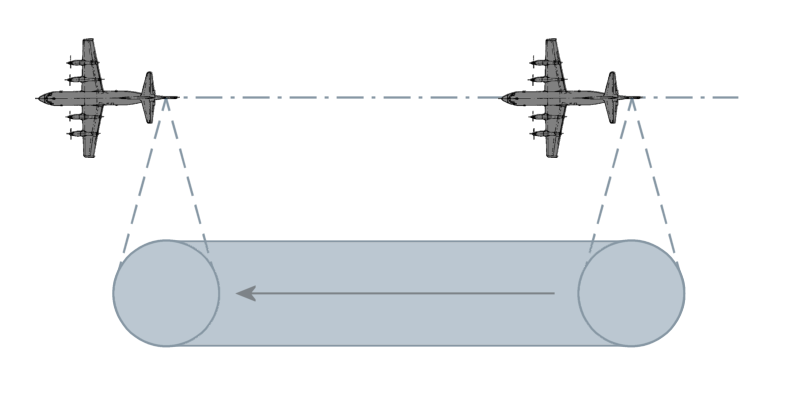
\includegraphics[width=0.45\linewidth]{../figures/sar_stripmap}	
	\caption{SAR in stripmap operation}
	\label{subfig:sar_stripmap}
	\end{subfigure}%
	\begin{subfigure}{.5\textwidth}
	\centering
	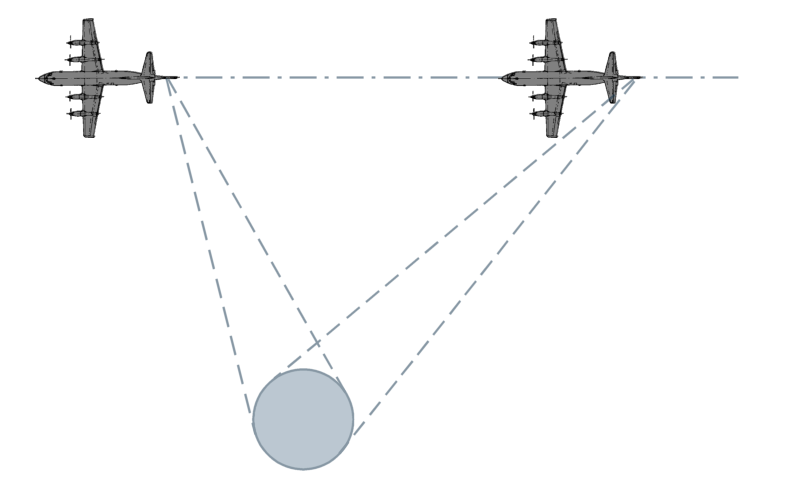
\includegraphics[width=0.45\linewidth]{../figures/sar_spotlight}	
	\caption{SAR in spotlight operation}
	\label{subfig:sar_spotlight}
	\end{subfigure}
	\caption{The two main modes of operation of SAR, reproduced from \cite{wolffSyntheticApertureRadar2012}}
	\label{fig:sar_modes}

\end{figure}

\subsubsection{The SAR radar equation}
There are two main approaches to SAR, focused and unfocused SAR. These differ in how they consider shifts in the response phase, as focused SAR only takes into account the Doppler shift across the aperture, while focused SAR takes into account the phase shift in the beam due to the change in range caused by the target passing through the beam. This means that the resolution of the image is determined by the length of the entire synthetic aperture, as opposed to in unfocused SAR where the resolution is a function of the shortest range between the platform and the target as well as the wavelength of the signal. The resolution of focused SAR is wavelength independent. The derivation of this can be found in Appendix \ref{appen:derivations}. Also in this appendix is a derivation of the radar equation both generally and then to the more specific version for SAR. The more general form of the radar equation for a single pulse is given as \[ \text{SNR} = \frac{P_t G^2 \lambda ^ 2 \sigma _b}{(4\pi)^3R^4kT_{sys} B} = \frac{P_t A_e^2 \sigma_b}{4\pi\lambda^2kT_{sys}BR^4}\] which gives the signal-to-noise ratio for a single pulse, where \gls{Pt} is the transmitted power, \gls{G} is the gain of the system, \gls{Ae} is the effective aperture area, \gls{lambda} is the wavelength of the signal, \gls{sigmab} is the radar cross-section, \gls{R} is the signal range, \gls{k} is Boltzmann's constant, \gls{Tsys} is the system noise temperature and \gls{B} is the bandwidth of the system. This can then be adapted to the SAR-specific radar equation by increasing the number of pulses \gls{n} to give \[\text{SNR} = \frac{P_t A_e^2 \sigma_b n}{4\pi \lambda^2kT_{sys}BR^4}\] and hence the signal-to-noise ratio of a distributed target is given by \[\text{SNR}=\frac{P_{av} A_e^2 \sigma^0\Delta R_g \Delta x t_{obs}}{4\pi\lambda^2kT_{sys}R^4} \text{     or     } \text{SNR} = \frac{P_{av}A_e^2\sigma^0\Delta x\lambda^3}{(4\pi)^3R^3kT_{sys}2v_p} \] where \gls{Pav} is the average power across all pulses, \gls{DeltaRg} is the ground range resolution of the system, \gls{tobs} is the observation time of the target and \gls{vp} is the platform velocity. The sensitivity of a SAR system can be expressed as the noise equivalent \gls{sigma0}, which is the value of \gls{sigma0} at the maximum range to give a signal-to-noise ratio of 1 (or 0 dB) \cite{watsonEE40136RadarSystems2020}.

\begin{figure}
\centering
\begin{subfigure}{.5\textwidth}
\centering
	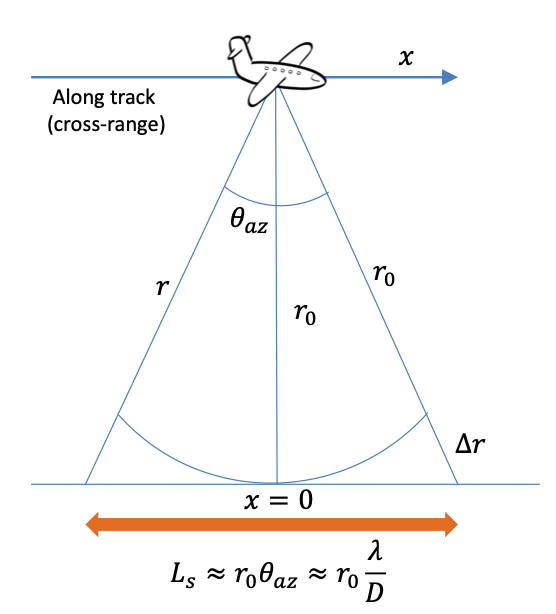
\includegraphics[width=0.9\linewidth]{../figures/sar_along_track_res}
\caption{Along-track/Cross-range SAR Resolution, reproduced from \cite{watsonEE40136RadarSystems2020}}
\label{subfig:sar_along_track}

\end{subfigure}%
\begin{subfigure}{.5\textwidth}
	\centering
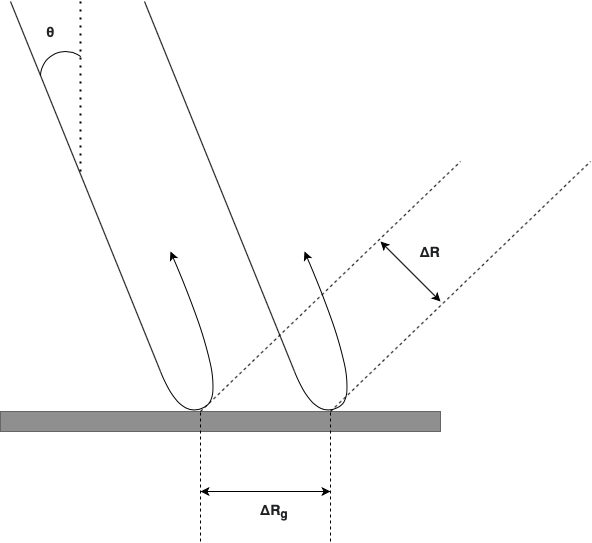
\includegraphics[width=0.9\linewidth]{../figures/down_range}	
\caption{Down-range SAR resolution, adapted from \cite{richardsRemoteSensingImaging2009}}
\label{subfig:down_range_SAR}
\end{subfigure}
\caption{Cross-sections of both dimensions of SAR range}
\label{fig:sar_range_cross_section}
\end{figure}


\subsubsection{SAR Image Artefacts}
There are a few artefacts that can arise as part of SAR imagery (and radar imagery in general). Some of these, such as range ambiguities, aren't relevant in this case due to the fact that all the targets being imaged are static and this is only a real issue in moving objects. Some artefacts will need to be considered though. The first of these is speckle, which is a result of the fact that the energy arriving at the pixel is pretty coherent, so it has a single phase on arrival at said pixel. Generally the pixel will be the sum of multiple scatterers as opposed to one single scatterer, meaning that it is likely to be affected by background reflections and so result in a relatively noisy image. This can be fixed in real world applications by splitting the SAR antenna into multiple sections and take the same image with each section. This then allows for the pixel values to be averaged out, hopefully removing the speckle at the cost of some resolution \cite{richardsRemoteSensingImaging2009}. \par 
Another image artefact that will need to be considered can be caused by strong scatterers that means that the signal is reflected multiple times before returning to the receiver. This can be seen most strongly with a bridge over water as it involves both a hard target in the bridge and a dihedral reflection from the water. This mostly occurs when the target is aligned with the path of the platform and the multiple reflections can cause the bridge to appear multiple times in the image due to the multiple bounces taken by the signal increase the Doppler shift presented when it is filtered on reception. The same signal is in essence received multiple times and so the algorithm reads it as different displacements for the same target \cite{richardsRemoteSensingImaging2009}. \par
Finally, some distortions can be created due to the geometry of the radar beam. Targets nearer the platform can appear compressed on the output image as the ground range in that location is greater but in the final image is represented in the same amount of image space as targets further away. Similarly, given a tower, reflections from the top of the tower will return to the platform before reflections from the bottom, causing the tower to appear to lean over towards the radar \cite{richardsRemoteSensingImaging2009}.

\section{Literature Review}

\subsection{A Summary of Methods Previously Explored in Literature}
The table that follows summarises the methods used in literature and a brief list of advantages and disadvantages. An in-depth exploration of the papers used can be found in section \ref{subsec:in_depth_findings} and an exploration of each possible method and their suitability for this project can be found in section \ref{sec:method_exploration}.
%TC:ignore
\begin{longtabu} to \textwidth {|X[0.5]|X|X|}
\hline

	Method & Advantages & Disadvantages\\
	\hline
	\endfirsthead
	\hline
	Method & Advantages & Disadvantages \\
	\hline 
	\endhead
	\hline
	\endfoot
	Raw signal & The most accurate method of simulation available as it uses the characteristics of the radar beam in order to simulate the responses of the structures it reflects off. & Most computationally complex method as it has to simulate the effects of every beam every time a pulse is transmitted and received. \\
	Rasterisation & The fastest method of simulating SAR as it uses image transformation techniques in order to give a good idea of how an image will look, this method is capable of real-time updates of the image which means it has applications in SAR data capture planning. & The least accurate method as it is only performing an image transform as opposed to a full simulation of the signal. \\
	Ray tracing & A good balance of speed and accuracy, uses advanced computer graphics techniques to only simulate the parts of the model available to the observer so is less computationally intense than the raw signal but also more accurate than rasterisation. & Requires a good graphics processor as well as a good modelling environment in which to perform it, this is by far the most complex to implement from scratch \\
	Hybrid methods & Has the potential to be a good balance between the raw signal and ray tracing as it uses raw signal for the higher order contributions and ray tracing for the more obvious single reflections & This is the least explored method so very few conclusions about its actual performance can be drawn, with only one paper found that uses it. \\
	
\end{longtabu}
%TC:endignore
\subsection{In-Depth Findings}
\label{subsec:in_depth_findings}
\subsubsection{Raw SAR Simulation}
There are three main methods that have previously been explored for simulating SAR. The first of these, which is the most accurate is simulating the effects of the beam itself, as detailed in Franceschetti \textit{et al.} 2003 \cite{franceschettiSARRawSignal2003}. This describes creating the raw data as would be expected in a SAR system in the real world and then transforming it to create a SAR image. The ground work for this was laid in Franceschetti \textit{et al.} 1992 \cite{franceschettiSARASSyntheticAperture1992}, which itself builds on Francescetti and Schirinzi's work on a SAR processor based on two-dimensional FFT codes \cite{franceschettiSARProcessorBased1990}. This approach has the advantages of being able to take into account backscattering as well as the higher-order signal contributions created by scattering as the signal reflects off of both a wall and the ground. A lot of the preliminary work with regards to the behaviour of electromagnetic backscattering was conducted in \cite{franceschettiCanonicalProblemElectromagnetic2002}. This describes a model that allows for the return from a structure to a microwave sensor to be analysed and so determine its dielectric properties as well as its geometric properties. The optics can be altered to simulate the roughness of the surface the signal is reflected off of last before it is received by the sensor. This can also be expanded to simulate backscattering. This simulator as a whole works very well with individual objects, however the simulation time was found to scale linearly with the number of objects present in the scene. Simulations in \cite{franceschettiSARRawSignal2003} were carried out using a Pentium IV processor from Intel Corp, released in 2001 which means that the simulation times achieved are not necessarily reflective of the performance achievable on more modern processors, however at the time it was found that while one object in a 512x512 pixel image required approximately 34 seconds, two objects in the same sized image required 1'02" and 16 objects increased this computation time up to 7'38". This is not ideal if the aim is real-time or even near real-time simulation capabilities as most urban environments that are to be simulated will contain far more than 16 structures. This efficiency does seem to have been improved in Franceschetti \textit{et al.} 2007 \cite{franceschettiSimulationToolsInterpretation2007} as in this paper it is used to simulate a SAR image of a $400\times 600 \textrm{m}^2$ area of the centre of Munich, incorporating the Technische Universität and the Alta Pinakothek, which leads to a reasonably complicated scene.  \par 
\begin{figure}
\centering
\begin{subfigure}{.5\textwidth}
	\centering
	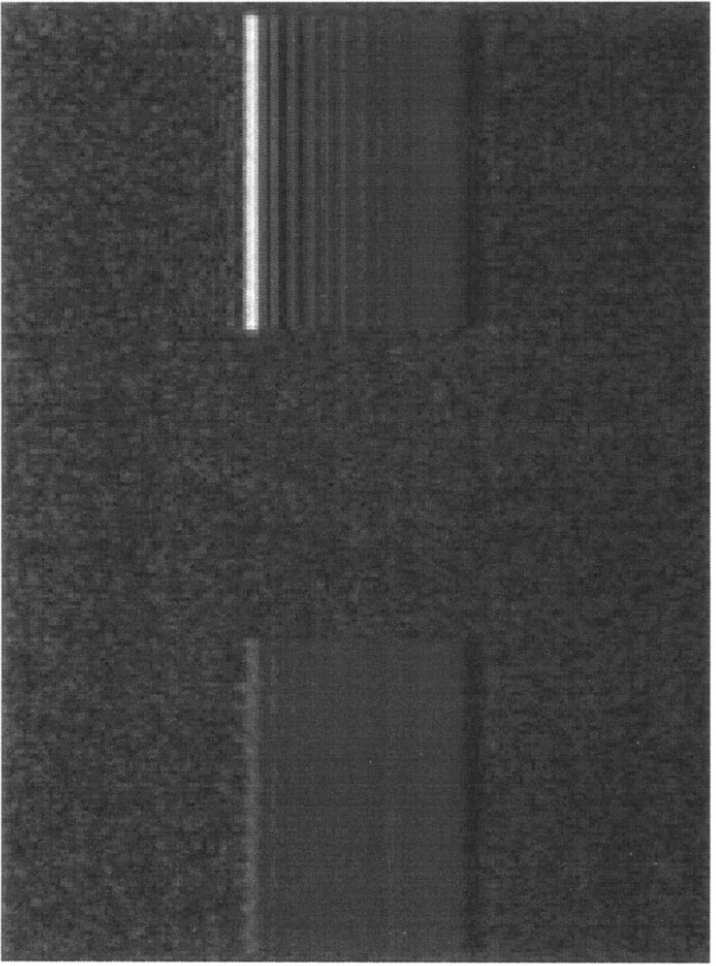
\includegraphics[width=0.9\linewidth]{../figures/franceschetti_2003_2_buildings}
	\caption{Simulated single-look SAR with two buildings}
	\label{fig:franceschetti_2003_2_buildings}
\end{subfigure}%
\begin{subfigure}{.5\textwidth}
	\centering
	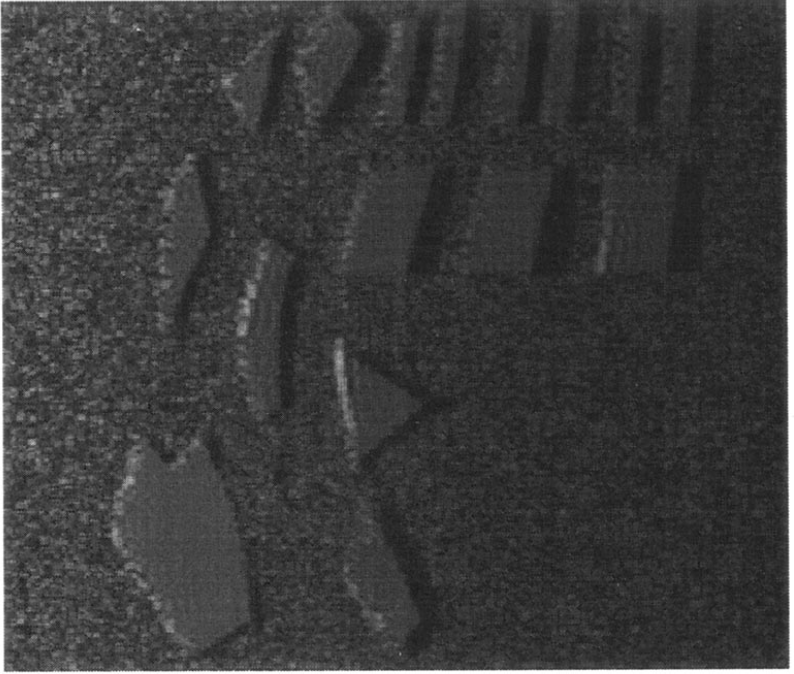
\includegraphics[width=0.9\linewidth]{../figures/franceschetti_2003_16_buildings}	
	\caption{Simulated single-look SAR with 16 buildings}
	\label{fig:franceschetti_2003_16_buildings}
\end{subfigure}
\caption{Simulated SAR images from Franceschetti \textit{et al.} 2003 \cite{franceschettiSARRawSignal2003}}
\label{fig:franceschetti_2003_buildings}
	
\end{figure}

\begin{figure}
\centering
\begin{subfigure}{.5\textwidth}
	\centering
	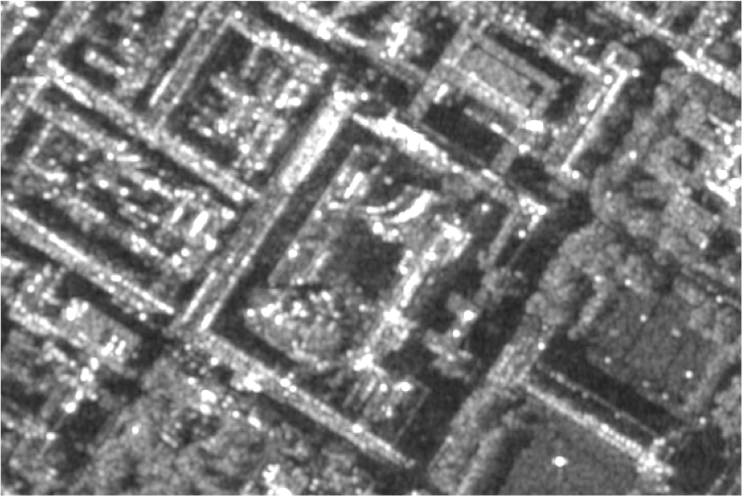
\includegraphics[width=0.9\linewidth]{../figures/franceschetti_2007_munich_sar}
	\caption{An actual SAR image of a portion of Munich}
	\label{fig:franceschetti_2007_munich_sar}
\end{subfigure}%
\begin{subfigure}{.5\textwidth}
	\centering
	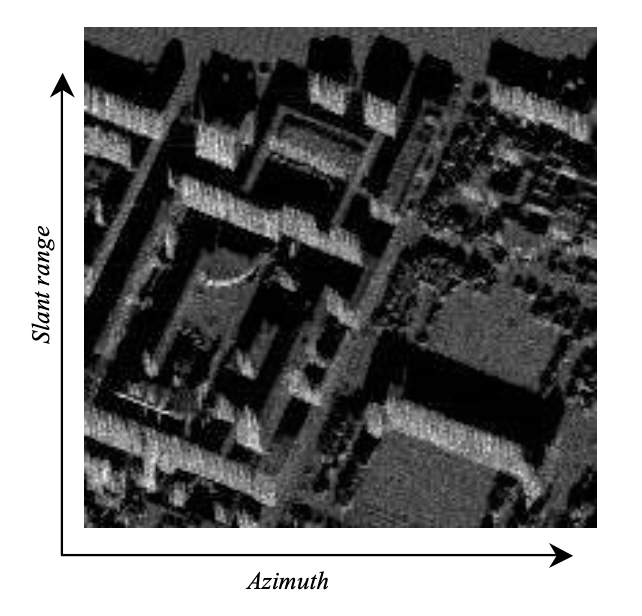
\includegraphics[width=0.9\linewidth]{../figures/franceschetti_2007_munich_sim}	
	\caption{A simulated SAR image of the same area}
	\label{fig:franceschetti_2007_munich_sim}
\end{subfigure}
\caption{A comparison between an actual SAR image and simulated SAR image of the Technische Universität and Alte Pinakothek from \cite{franceschettiSimulationToolsInterpretation2007}}
\label{fig:franceschetti_2007_munich}
	
\end{figure}

A similar approach building on the previously mentioned work is presented by Zheng \textit{et al.} \cite{zhengSimulationMethodSAR2008} which uses the scattering model in order to accurately simulate a SAR scene. This is achieved by making the assumption that the scene is made up of vertical buildings distributed on a rough dielectric terrain. This also discusses the computation of scattering coefficients under different conditions. As with the previous approach (and the following raw SAR approach) the Kirchhoff approach is used in this case.
\par
A similar approach to robust SAR simulation is described in Dellière \textit{et al.} 2007 \cite{delliereSARMeasurementSimulation2007}, which uses an electromagnetic approach closely following Maxwell's equations to create a finite-difference time domain method of simulation, which differs from \cite{franceschettiSARRawSignal2003} as that instead manipulates the signal in the frequency domain in order to create the raw SAR signal. This system has similar drawbacks to Franceschetti's approach with regards to computation complexity and time required, but is even more computationally complex, due to its ability to handle dispersive materials as well as phase changes. This approach could be of some interest for creating an incredibly robust simulator due to the advances in computing performance between the publication date and today. \par
\subsubsection{Graphical SAR Simulation}
There are two methods that are less complex computationally for simulating the image achieved by SAR. These both arise from graphics manipulation and more specifically 3 dimensional modelling. These are rasterisation and ray tracing. Rasterisation is the process of taking a 3 dimensional area and creating a 2 dimensional image using some sort of image transformation based on the location of the camera to the object in the 3D area. Ray tracing follows a similar process to light, just in reverse. It sends beams out from the camera in all directions that the camera can see and simulates them reflecting off of objects until they hit a source of illumination. Using this the rendering engine can determine if an object is illuminated or not and adjust appropriately. These two approaches have both been used in the past for simulation of SAR images. Rasterisation was used by Balz 2006 \cite{balzRealtimeSARSimulation2006} and ray tracing was explored by Auer \textit{et al.} 2008 \cite{auerRayTracingSimulating2008} and Mametsa \textit{et al.} 2002 \cite{mametsaImagingRadarSimulation2002}. This second paper was used in Hammer \textit{et al.} \cite{hammerComparisonSARSimulation2008} along with Balz 2006 to compare the relative merits of these two approaches. Ultimately the advantages of Balz's approach as detailed in \cite{balzImprovedRealTimeSAR2006} and \cite{balzRealtimeSARSimulation2006} is that the simulator is real-time so can be used to determine optimal azimuthal directions when recording a SAR image using a physical airborne platform. This form of simulation however doesn't take into account the contributions of higher order reflections so if it is being used for a demonstration tool, the images produced are less representative of an actual SAR image. This also means that corners aren't visible in the image, meaning that this form of simulation can't be used to test feature extraction algorithms. The two ray tracing simulators tested within \cite{hammerComparisonSARSimulation2008} can simulate these higher-order contributions meaning they can be used to test feature extraction algorithms, however due to the computationally intensive nature of ray tracing these can't be simulated in real time, so this form of simulation is less useful for planning purposes. \par
\begin{figure}
\centering
\begin{subfigure}{.5\textwidth}
	\centering
	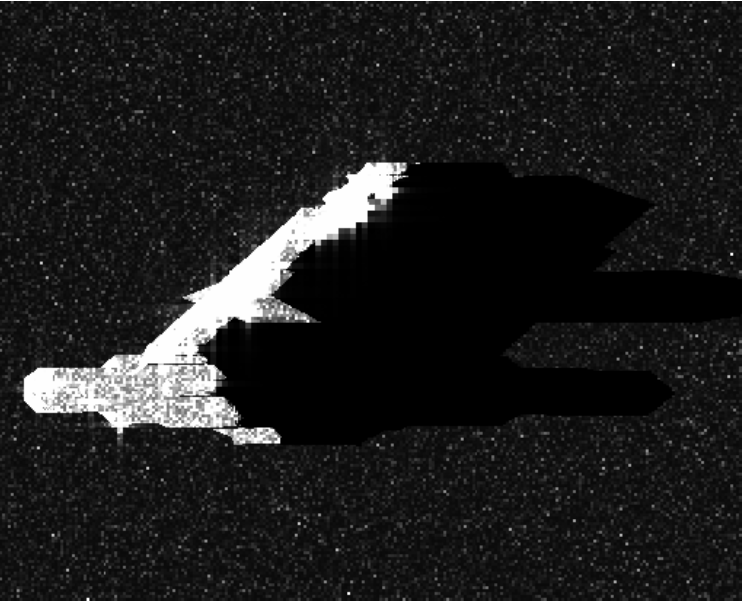
\includegraphics[width=0.9\linewidth]{../figures/balz_2006_stiftskirche}
	\caption{0.3m resolution simulation of the Stiftskirche in Stuttgart}
	\label{fig:balz_2006_stiftskirche}
\end{subfigure}%
\begin{subfigure}{.5\textwidth}
	\centering
	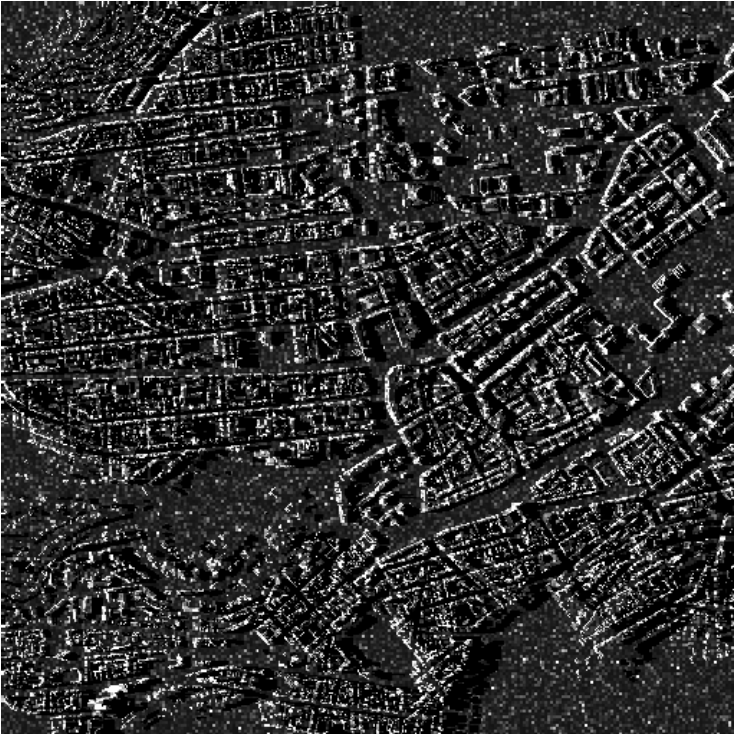
\includegraphics[width=0.9\linewidth]{../figures/balz_2006_stuttgart}	
	\caption{5m resolution simulation of Stuttgart}
	\label{fig:balz_2006_stuttgart}
\end{subfigure}
\caption{Results from Balz 2006 \cite{balzImprovedRealTimeSAR2006} using rasterisation techniques}
\label{fig:balz_2006_images}
	
\end{figure}

\begin{figure}
\centering
\begin{subfigure}{.5\textwidth}
	\centering
	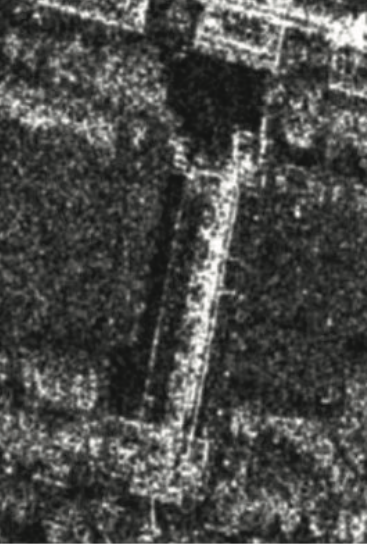
\includegraphics[width=0.9\linewidth]{../figures/auer_2008_terrasar_ref}
	\caption{A reference spotlight image of the Alta Pinakothek}
	\label{fig:auer_2008_ref}
\end{subfigure}%
\begin{subfigure}{.5\textwidth}
	\centering
	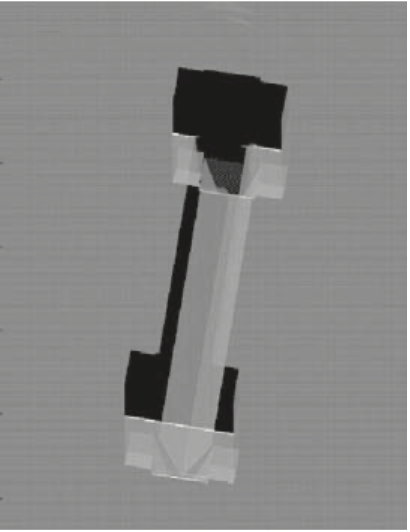
\includegraphics[width=0.9\linewidth]{../figures/auer_2008_all_reflections}	
	\caption{A simulated SAR image using ray tracing of the Alta Pinakothek}
	\label{fig:auer_2008_all}
\end{subfigure}
\caption{Simulated SAR using ray tracing from Auer \textit{et al.} 2008 \cite{auerRayTracingSimulating2008}}
\label{fig:auer_2008_ray_tracing}
	
\end{figure}


All of the forms of simulation presented here so far are only as good as the models used, as generally the modelled buildings are assumed to be made of one material with a fixed dielectric constant, while the modelled ground is made of a different material. In \cite{hammerComparisonSARSimulation2008}, the buildings modelled are created entirely of stone, with a grass ground. In real life however this becomes more complicated as buildings do tend to be made up of multiple materials, and often in urban areas the ground is made up of a material with a similar dielectric constant to the buildings. This also doesn't include any forms of dispersive materials such as metal. It is unclear whether any of the simulators covered in \cite{hammerComparisonSARSimulation2008} can simulate these sorts of materials accurately, which is something that should be taken to account in the future. \par
Yet another method similar to the image processing approaches is presented by Lu \textit{et al.} \cite{luGPUBasedRealtime2009} and uses methods most commonly used by video games. In this case the raw mathematic SAR simulation is not carried out, similar to \cite{balzHybridGPUBasedSingle2009} and \cite{auerRayTracingSimulating2008} and uses an orthogonal projection to cast the 3D model to a 2D image based on the slant range of the camera. This again has the potential of improving the performance of image generation in incredibly complicated scenes such as city centres.
\par 
\subsubsection{Hybrid Method and Other Papers of Note}
Chen \textit{et al.} 2011 \cite{chenRadarImagingSimulation2011} proposes a hybrid method of simulating these images using analytical models. In this approach, the contributions provided by backscattering are shown using an electromagnetic analytical model ultimately based on that described by \cite{franceschettiSARRawSignal2003}, and the object position vectors are given by a geometric model using ray tracing. In this paper the analysis is mostly focused on cylindrical or cylinder-like buildings, with some analysis devoted to flat-roof buildings as well. This approach has a potential to be more accurate than the ray tracing models proposed previously due to the electromagnetic models involved, but also be less computationally complex than the more canonical SAR image simulators. 
\par
Xu and Jin 2006 \cite{xuImagingSimulationPolarimetric2006} is a paper that is not immediately relevant to this situation due to it modelling natural environments for SAR simulation however this is potentially interesting and relevant due to the variety of materials present in urban environments to be modelled. This is an algorithm that can deal with randomly and heterogeneously distributed objects within an image with varying dielectric constants and can deal with them in a reasonable length of time. This is something that is worth exploring if there is time in the future as it would add robustness to the system as a whole. 







\chapter{Methods}
\section{Exploration of Potential Methods and Their Suitability}
\label{sec:method_exploration}
The four possible methods that can be used in this project are, as mentioned previously, raw signal simulation, rasterisation, ray tracing and a hybrid method. In this section I will cover their suitability as they relate to this project, as well as explore the methods of transforming SAR raw signals into an image.
\subsection{SAR Simulation Methods}
\subsubsection{Raw SAR Simulation}
This is the most robust form of simulation and the most accurate as the individual signals are simulated as well as their reflections. This does have some drawbacks as developing the system in the first place is likely to be quite complex. This system requires the implementation of a transmission and reception element (likely to be two separate functions for complexity reasons), a free-space element, an element to act as the target would in real life to accurately simulate the return signal, some sort of coordinate system to position both the target and the platform in free space and finally the linear FM waveform. These are all sections that, while the conceptual understanding of their operation is relatively easy to grasp given prior knowledge of how wireless communications and more specifically radar work, are not altogether simple in their implementation. Fortunately this would not be implemented blind thanks to Franceschetti \textit{et al.} 2003 \cite{franceschettiSARRawSignal2003} and all the foundational work that led to it however this work has been refined over the course of more than a decade, not several weeks, which is potentially the biggest limitation on how in-depth this implementation can go and the biggest roadblock against this particular method of simulation. 
\subsubsection{Rasterisation}
As previously mentioned, rasterisation is one approach to SAR simulation that does not require lengthy implementation processes as rasterisation is a standard process in image manipulation. In this case what would be required is devising some sort of transform from the 3-dimensional image simulated and the SAR output. This will not be true SAR as it is only the result of taking one image from one place and therefore will not truly be an accurate representation. As was discussed in Balz 2006 \cite{balzImprovedRealTimeSAR2006} and all related work this is a desirable outcome in the event that this SAR simulation is to be used as a real-time simulation in order to plan actual SAR imaging flights. In this project this isn't necessarily the case as my intention is to create a final product that is usable as a teaching aide, which would involve some sort of progression as the SAR image is taken. This isn't a particularly practical approach to be used with this in mind as it can be done instantly (or as near as to a human) and the image isn't built up over multiple measurements.
\subsubsection{Ray-tracing}
Ray-tracing is, in this case, somewhat of a hybrid method. As it doesn't simulate the free space and electromagnetic effects of the radar it isn't truly SAR however it works in a similar just inverted way. This is because the light beams (here analogous to the higher frequency EM waves) are projected from the observer (the receiver) and reflect off objects until they reach a source of illumination (the transmitter). This could be useful for teaching purposes as the method by which it works could be the same and then the image is built using similar image formation methods to those used by true SAR. The issue with this type of simulation is a relative lack of experience in it and some issues with the complexity of implementation. This is partially an issue with all three forms of simulation which will be covered in the following section, but also ray-tracing is known to be a very computationally intense form of visual rendering and requires a strong knowledge with three-dimensional rendering techniques to even begin to implement a version of this.
\subsubsection{True Hybrid Methods}
This would probably be the most complex path to take as it would require choosing two of the above methods and combining them in an as yet mostly unexplored way. This would run most heavily into the issues laid out in section \ref{sec:3drender} as it would require heavily editing the 3D rendering engine chosen to be able to perform the necessary simulations which would reduce computing resources required in the long run but would possibly require more work than is possible during the ten weeks allotted to this project.
\subsubsection{3D Rendering Engines}
\label{sec:3drender}
There is a problem common to all three of these potential methods, which is that no matter what they will require some form of 3D rendering engine, either to simulate the effect of the radar waves or ray-tracing, or to provide a 3D image base for the rasterisation transformation. Unsurprisingly none of the rendering engines currently commonly available are perfectly suited for this and many of the ones investigated were unusable for this case. Ideally some time would be allowed for creating a custom 3D modelling engine that would properly handle EM waves or equivalent. The closest to being feasible for this application appeared to be Blender \cite{foundationBlenderOrgHome}, an incredibly powerful modelling engine released under a GNU Public License by the Blender Foundation that has a Python scripting engine, however due to a lack of familiarity with this software it was decided that gaining a strong enough familiarity with the package would take too long to be practical in this project. The final approach chosen is discussed in Section \ref{subsec:approach_chosen}
%TODO extend these somewhat
\subsection{Image Forming Methods}
Raw SAR simulation requires an image formation method. This takes the overlapping received signals and time-multiplexes them to display an image that can be interpreted by a person, especially with multiple targets at the same range. There are multiple forms available and a few of them will be discussed here. These will all be the forms used for airborne (including space-based) platforms as there are some corrections required for ground-based systems that are irrelevant here although are covered in Guo and Dong (2016) \cite{guoModifiedOmegaKAlgorithm2016}, as well as in a practical sense on the blog of Henrik Forstén for both an Omega-K \cite{forstenSyntheticapertureRadarImaging2019} and Backprojection \cite{forstenBackprojectionBackpropagation2019} approach (both covered here, among others). All the algorithms will operate in similar ways however they all have strengths and weaknesses. 
\subsubsection{\gls{oka}}
Omega-K is otherwise known as the range migration algorithm. It works by first Fourier transforming the received SAR signal into the frequency domain and then performing bulk compression, which is where the signal is multiplied by a reference function computed for a known range. A target is correctly focused at this reference range but targets not at this range are only partially focused. Following this, the signal undergoes Stolt interpolation, which re-maps the range frequency axis in order to bring targets away from the reference range into focus. It achieves this by transforming the range frequency so the phase is linear. This effectively removes all phase terms higher than the linear term, although these aren't ignored. Finally an inverse Fourier transform is performed on the signal to put it back into the image domain. For a more in depth explanation of how the Stolt mapping works, see Cumming \textit{et al.} 2003 \cite[section~3]{cummingInterpretationsOmegaKAlgorithm2003}. This approach does assume that the trajectory is completely straight so if this isn't achieved then the displayed image will be incorrect \cite{albuquerqueApplicationsTimeDomainBackProjection}. For this application this is not an issue of concern as the simulated airborne platform will always be travelling in a straight line but is worth keeping in mind for more general applications.
\subsubsection{Backprojection}
Backprojection uses a matched filter approach to get the difference between the expected return from the radar and the actual return from the radar and was originally developed for use in computer-aided tomography for medical reasons \cite{naComparisonBackProjectionRange2006}. This is generally performed in the time domain as opposed to the frequency domain due to the lack of assumptions that have to be made \cite{albuquerqueApplicationsTimeDomainBackProjection}. The way this works is the position of the platform is known in 3 dimensional space and so the expected return can be calculated based on the time delay from the reflected signal. The matched filter that this creates can then remove this from the received signal and the difference is due to an object that reflected the signal prematurely. There are some other sources of error in this case such as multiple bounces on the image or impreciseness in calculating the imaging platform position \cite{duerschBackprojectionSyntheticAperture2013}. This algorithm is not ideal as it is very computationally intensive and requires that the imaging geometry needs to be precisely known. This positioning can normally be estimated using an inertial navigation system so is not particularly difficult to obtain however it does need to be precise as this can make received images appear shifted from where they are actually positioned. As each pixel can be handled independently of the other pixels it is ideally suited for parallel computing so the computation time can be reduced significantly \cite{albuquerqueApplicationsTimeDomainBackProjection}.
\subsubsection{\gls{rda}}
This algorithm is similar in process to $\omega KA$. It is implemented in the frequency domain but operates only in one dimension at a time, which improves the simplicity of the algorithm. The first step is range migration, which is where the raw data is Fourier transformed in the range dimension and multiplied with the range reference signal and transforms back to the image domain. This algorithm then performs a Fourier transform in the azimuth only, transforming to the range Doppler domain before performing a \gls{rcmc}. This is to correct for the slant range to the target changing as the platform moves through space, meaning that the Doppler frequency of the target is different at different times and so appears at different ranges. The RCMC corrects for this by shifting each cell a set number of metres depending on its distance from the reference range \cite{parasharStudyRangeCell2015}. After this a matched filter for just the azimuth is used to perform azimuth compression and the whole image is returned to the image domain for visualisation \cite{dastgirProcessingSARData2007}. This algorithm was created in the 1970s and so is more basic than the Omega-K algorithm. In this case the RDA in an accurate form is somewhat equivalent to an approximate form of $\omega KA$, however RDA is often used in a less accurate form where the range compression is not varied according to either range or azimuth frequencies, and the accurate form of $\omega KA$ is more accurate than the approximate form \cite{cummingInterpretationsOmegaKAlgorithm2003}, so is a better choice for this application.
\subsubsection{\gls{csa}}
Chirp scaling is quite similar to RDA, and the difference is improving the RCMC by removing the interpolation required. It does this by applying a phase multiply in order to equalise the range migrations of all the targets. This Chirp scale factor is generally 1 for a satellite based SAR system and higher for aircraft based \cite{dastgirProcessingSARData2007}. This algorithm has an accuracy somewhere between that of the accurate and approximate $\omega KA$ and approximate $\omega KA$ is  roughly equivalent to CSA if there was no chirp scaling performed \cite{cummingInterpretationsOmegaKAlgorithm2003}.
\subsection{Discussion of Approaches Chosen and Reasoning}
\label{subsec:approach_chosen}
After carefully considering the approaches discussed above, the decision has been made to implement the SAR simulation using raw methods, specifically using the Simulink Phased Array Toolbox, with image formation performed using MATLAB. This is because the issues with implementing all the sections mentioned previously are removed and they are created in a far more robust way than would be possible to implement within the time available for this project. Simulink has been chosen for this because it's more tactile than the equivalent MATLAB code would be so is better for the desired outcome in this case which is to create a tool that can be used as a teaching aid while learning synthetic aperture radar. Simulink also gives access to the Simulink 3D Animation Toolbox, which allows for linking models to a 3D visualisation, which is similarly useful in a teaching environment. Simulink is not suited to image formation algorithms as they require all the data to be present at once, whereas Simulink works best when the data can be fed in over the length of the simulation. Therefore these will be implemented in MATLAB. In this case, both $\omega KA$ and backprojection will be implemented as the differences between the two will be interesting to observe, especially considering the data input will be identical. These have been chosen as they are more accurate than either CSA or RDA and so will give a better representation. Specifically $\omega KA$ will be implemented using the accurate version described in Cumming \textit{et al.} 2003 \cite{cummingInterpretationsOmegaKAlgorithm2003} and backprojection will be implemented based on the efficient approach outlined in Yegulalp 1999 \cite{yegulalpFastBackprojectionAlgorithm1999} as this should be simpler to implement than more standard backprojection algorithms, especially as the steps are very kindly laid out within the paper. The way this version of backprojection works is by dividing the full aperture into subapertures and generating an image in each of the subapertures. These can then all be recombined by coherently summing all the images into the final image. All of the subapertures are quite coarse in the cross-range direction which reduces the number of operations required and then they can be upscaled when they are combined back into the full image. 
\section{Desired Results and Outcomes}
The major desired outcome of this project is to have a Simulink model that can simulate a SAR system with one target, in such a way that it can be easily examined for teaching purposes. This model must output data so that a MATLAB script can read it in and perform at least one and more ideally two methods of image formation. This Simulink model must also feed into a Simulink 3D World in such a way that it is obvious what is happening in the model and provide a visual aid to the model when it is running. Extended from this it would be ideal if the dimensions of the target could be read in from the Simulink 3D World and used to update the \gls{rcs} of the target within the Simulink model in a dynamic fashion. As another extension to this, a cone to visualise the antenna beam within the Simulink 3D World would be nice to have however is not completely necessary. Finally, the ability within the model to switch between stripmap and spotlight modes and have the cone within the 3D World update to match would be nice however again not strictly necessary. 
\section{Milestones}
These milestones have been revised from the original milestones as set out in the interim report \cite{moffatSyntheticApertureImaging}. This is due to an increase in understanding of the requirements of the project and an updated schedule. 
%TC:ignore
\begin{longtabu} to \textwidth {|X[0.5]|X|}
\hline

	Milestone & Description\\
	\hline
	\endfirsthead
	\hline
	Milestone & Description \\
	\hline 
	\endhead
	\hline
	\endfoot
	1 - Basic Model & The first milestone is to have a SAR system model that outputs data in a usable format and can be visualised using a MATLAB plot function. The target in this case can be just a spot target with a high average radar cross section as the realism is not a worry in this case.  \\
	2 - Basic Image Formation & In this milestone the aim is to convert the data output by the model in Milestone 1 to a visible image using some form of image formation algorithm. This can be either \glsxtrshort{oka} or backprojection, although it will most likely be \glsxtrshort{oka} due to the comparative simplicity in implementation when compared to backprojection. The other will be implemented following Milestone 3 as it is less important to have two different image formation algorithms than this step. \\
	3 - Basic Reference Model & Milestone 3 is to implement a 3 dimensional representation of the process that is occurring in the model. At this stage the only real requirement is to have a representation of the airborne platform and a representation of the target in the correct places for a given point in the simulation. This will also include the platform moving at an accurate rate past the target. \\
	4 - Completed Image Formation & The aim of this milestone is to finish the image formation algorithms selected for use in this model by implementing whichever algorithm is not created in milestone 2. \\
	5 - Simulink Model Improvements & The aim of this milestone is to implement the other major form of SAR to that created in milestone 1, whether that is stripmap or spotlight and to include a method of being able to display the results of both forms of SAR at one time or another. The form that this will take is yet to be decided. \\
	6 - 3D Model Improvements & Improve the amount of information imparted by the 3D model for an educational environment by representing the antenna beam or similar \\
	7 - Immersiveness & Use a calculated radar cross section of the target to improve the image while also displaying this target within the 3D environment \\
	
\end{longtabu}
%TC:endignore










































\chapter{Deliverables}
\section{Deliverables Achieved}
\section{Significant Results}
\section{Uncertainty}
\section{Final Results}
\chapter{Conclusions}
\section{Final Remarks and Outcome}
\section{Further Work}
\newpage
\section*{Acknowledgements}
\printbibliography

%TC:ignore
\appendix
\chapter{Derivations}
\label{appen:derivations}
\section{Focused SAR Resolution}
\subsection{Along track resolution}
\begin{gather}
	r = r_0 + \Delta r \\
	\Delta r = (r_0^2 + x^2) ^ \frac{1}{2} - r_0\\
	\Delta r \approx \frac{x^2}{2r_0}\\
	\phi(x) = -2k_0 \Delta r = -\frac{2\pi x^2}{\lambda r_0}\\
	\theta _{sa} \approx \frac{\lambda}{2L_s}\\
	\Delta x = \theta _{sa}r_0\\
	\Delta x = \frac{\lambda}{2L_s}r_0 = \frac{\lambda}{2r_0\frac{\lambda}{D}} r_0\\
	\Rightarrow \Delta x = \frac{D}{2}
\end{gather}
In this case, \gls{r} is the outer radial distance of the beam, \gls{r0} is the center distance of the beam, \gls{deltar} is the difference between these two distances, \gls{x} is the distance travelled by the platform over the time measured, \gls{k0} is the angular wave number of the signal, \gls{phix} is the two-way phase history of the signal, \gls{lambda} is the wavelength of the signal, \gls{thetasa} is the synthesised beam width obtained after azimuth processing, \gls{deltax} is the resolution of the system and \gls{D} is the aperture size in the chosen dimension (i.e. here it's the azimuthal dimension). Derivation from \cite{richardsRemoteSensingImaging2009} and \cite{watsonEE40136RadarSystems2020}.
\subsection{Down-range resolution}

With the assumption made that there is some form of pulse compression on the signal we have a radial resolution of \[\Delta R = \frac{c}{2B}\] and by geometry we get a ground resolution of \[\Delta R_g = \frac{c}{2B\sin(\theta)}\] so to avoid any range ambiguities, \[\frac{c}{2R_{max}} > \text{PRF} \] where \gls{Rmax} is the maximum range achievable by the radar, \gls{DeltaRg} is the ground range resolution and \gls{DeltaR} is the radial resolution of the signal.
\section{Derivation of the Radar Equation}
Again derivations from \cite{richardsRemoteSensingImaging2009} and \cite{watsonEE40136RadarSystems2020}. \begin{gather}
 \text{Isotropic Antenna Power Density} = \frac{P_t}{4\pi R^2}\\
 \text{Directive Antenna Power Density} = \frac{P_tG_t}{4\pi R^2}\\
 \text{Power Intercepted by Target} = \frac{P_tG_t}{4\pi R^2}\sigma_b\\
 \text{Power density at receiver} = \frac{P_tG_T}{4\pi R^2}\sigma_b \times \frac{1}{4\pi R^2}\\
 P_r = \frac{P_tG_t}{4\pi R^2} \sigma_b \times \frac{1}{4\pi R^2} \times A_e \\
 G_r = \frac{4\pi}{\lambda^2}A_e\\
 G_t = G_r = G \\
 \Rightarrow P_r = \frac{P_tG^2\lambda^2}{(4\pi)^3R^4}\sigma_b
 \end{gather}
 Noise power \gls{Pn} is given by $P_n = kT_{sys}B$ and so the equation for SNR is given as \[ \frac{P_r}{P_n} = \frac{P_tG^2\lambda^2\sigma_b}{(4\pi)^3R^4kT_{sys}B}\] and so the radar equation for a distributed target is given by 
 \begin{gather}
 \sigma_b = \sigma^0 \Delta R_g \Delta x \\
 	\Delta x = \frac{R\lambda}{2L_s} = \frac{D}{2}\\
 	\Delta R_g = \frac{c}{2B\sin(90\degree - \alpha)}\\
 	t_{obs} = nT_s = \frac{L_s}{v_p}\\
 	n = \frac{L_s}{T_sv_p}\\
 	P_t = \frac{P_{av}T_s}{\tau}\\
 	\tau B \approx 1\\
 	\text{SNR}=\frac{P_{av}A_e^2\sigma^0\Delta R_g\Delta x t_{obs}}{4\pi\lambda^2kT_{sys}R^4} \text{or} \text{SNR} = \frac{P_{av}A_e^2\sigma^0\Delta x\lambda^3}{(4\pi)^3R^3kT_{sys}2v_p}
 \end{gather}


\chapter{Code Listings}
\label{appen:listings}
\section{trigger\_script.m}
\inputminted[breaklines]{matlab}{../blender/trigger_script.m}
\label{lst:trigger_script}
%TC:endignore
\end{document}